


\tikzset{every picture/.style={line width=0.75pt}} %set default line width to 0.75pt        

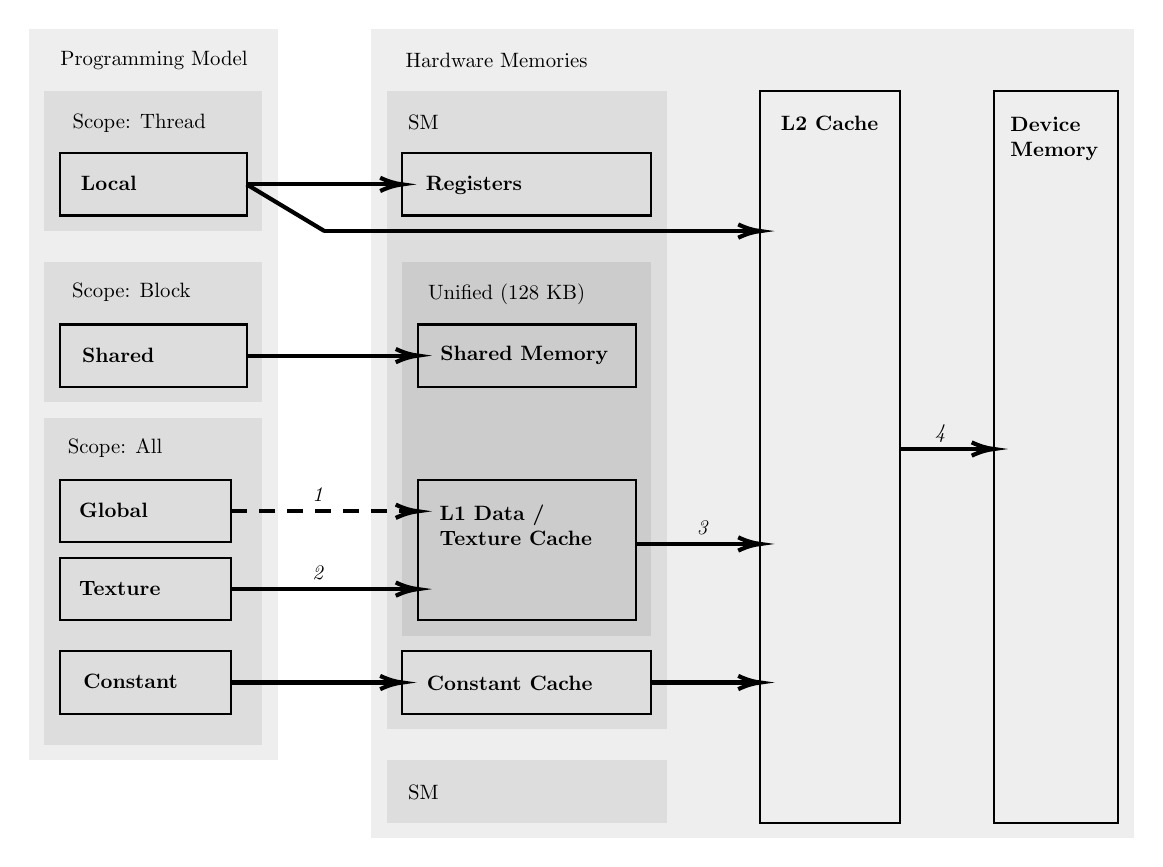
\begin{tikzpicture}[x=0.75pt,y=0.75pt,yscale=-0.75,xscale=0.75, every node/.style={scale=0.75}]
%uncomment if require: \path (0,574); %set diagram left start at 0, and has height of 574

%Shape: Rectangle [id:dp49466026838319044] 
\draw  [draw opacity=0][fill={rgb, 255:red, 238; green, 238; blue, 238 }  ,fill opacity=1 ] (10,10) -- (170,10) -- (170,480) -- (10,480) -- cycle ;
%Shape: Rectangle [id:dp28817003892392545] 
\draw  [draw opacity=0][fill={rgb, 255:red, 221; green, 221; blue, 221 }  ,fill opacity=1 ] (20,50) -- (160,50) -- (160,140) -- (20,140) -- cycle ;
%Shape: Rectangle [id:dp36092800198336605] 
\draw   (30,90) -- (150,90) -- (150,130) -- (30,130) -- cycle ;
%Shape: Rectangle [id:dp731633578877624] 
\draw  [draw opacity=0][fill={rgb, 255:red, 221; green, 221; blue, 221 }  ,fill opacity=1 ] (20,160) -- (160,160) -- (160,250) -- (20,250) -- cycle ;
%Shape: Rectangle [id:dp9265995086938097] 
\draw   (30,200) -- (150,200) -- (150,240) -- (30,240) -- cycle ;
%Shape: Rectangle [id:dp7383874820875151] 
\draw  [draw opacity=0][fill={rgb, 255:red, 221; green, 221; blue, 221 }  ,fill opacity=1 ] (20,260) -- (160,260) -- (160,470) -- (20,470) -- cycle ;
%Shape: Rectangle [id:dp3490802882861901] 
\draw   (30,300) -- (140,300) -- (140,340) -- (30,340) -- cycle ;
%Shape: Rectangle [id:dp7130701095363465] 
\draw   (30,410) -- (140,410) -- (140,450) -- (30,450) -- cycle ;
%Shape: Rectangle [id:dp4095820299975792] 
\draw   (30,350) -- (140,350) -- (140,390) -- (30,390) -- cycle ;
%Shape: Rectangle [id:dp6482924830961656] 
\draw  [draw opacity=0][fill={rgb, 255:red, 238; green, 238; blue, 238 }  ,fill opacity=1 ] (230,10) -- (720,10) -- (720,530) -- (230,530) -- cycle ;
%Shape: Rectangle [id:dp1781724326419385] 
\draw  [draw opacity=0][fill={rgb, 255:red, 221; green, 221; blue, 221 }  ,fill opacity=1 ] (240,50) -- (420,50) -- (420,460) -- (240,460) -- cycle ;
%Shape: Rectangle [id:dp7630031584827657] 
\draw   (250,90) -- (410,90) -- (410,130) -- (250,130) -- cycle ;
%Shape: Rectangle [id:dp2432538926228578] 
\draw  [draw opacity=0][fill={rgb, 255:red, 204; green, 204; blue, 204 }  ,fill opacity=1 ] (250,160) -- (410,160) -- (410,400) -- (250,400) -- cycle ;
%Shape: Rectangle [id:dp1012169215247074] 
\draw   (630,50) -- (710,50) -- (710,520) -- (630,520) -- cycle ;
%Shape: Rectangle [id:dp4402700694413979] 
\draw  [draw opacity=0][fill={rgb, 255:red, 221; green, 221; blue, 221 }  ,fill opacity=1 ] (240,480) -- (420,480) -- (420,520) -- (240,520) -- cycle ;
%Shape: Rectangle [id:dp927031941414987] 
\draw   (480,50) -- (570,50) -- (570,520) -- (480,520) -- cycle ;
%Shape: Rectangle [id:dp46907454808635207] 
\draw   (250,410) -- (410,410) -- (410,450) -- (250,450) -- cycle ;
%Shape: Rectangle [id:dp03098174365738804] 
\draw   (260,200) -- (400,200) -- (400,240) -- (260,240) -- cycle ;
%Shape: Rectangle [id:dp8107477823122851] 
\draw   (260,300) -- (400,300) -- (400,390) -- (260,390) -- cycle ;
%Straight Lines [id:da27581340197107873] 
\draw [line width=1.5]    (150,110) -- (247,110) ;
\draw [shift={(250,110)}, rotate = 180] [color={rgb, 255:red, 0; green, 0; blue, 0 }  ][line width=1.5]    (14.21,-4.28) .. controls (9.04,-1.82) and (4.3,-0.39) .. (0,0) .. controls (4.3,0.39) and (9.04,1.82) .. (14.21,4.28)   ;
%Straight Lines [id:da7214512267404303] 
\draw [line width=1.5]    (200,140) -- (477,140) ;
\draw [shift={(480,140)}, rotate = 180] [color={rgb, 255:red, 0; green, 0; blue, 0 }  ][line width=1.5]    (14.21,-4.28) .. controls (9.04,-1.82) and (4.3,-0.39) .. (0,0) .. controls (4.3,0.39) and (9.04,1.82) .. (14.21,4.28)   ;
%Straight Lines [id:da2675628197899167] 
\draw [line width=1.5]    (150,110) -- (200,140) ;
%Straight Lines [id:da1581409251714272] 
\draw [line width=1.5]    (150,220) -- (257,220) ;
\draw [shift={(260,220)}, rotate = 180] [color={rgb, 255:red, 0; green, 0; blue, 0 }  ][line width=1.5]    (14.21,-4.28) .. controls (9.04,-1.82) and (4.3,-0.39) .. (0,0) .. controls (4.3,0.39) and (9.04,1.82) .. (14.21,4.28)   ;
%Straight Lines [id:da2900127660824916] 
\draw [line width=1.5]  [dash pattern={on 5.63pt off 4.5pt}]  (140,320) -- (257,320) ;
\draw [shift={(260,320)}, rotate = 180] [color={rgb, 255:red, 0; green, 0; blue, 0 }  ][line width=1.5]    (14.21,-4.28) .. controls (9.04,-1.82) and (4.3,-0.39) .. (0,0) .. controls (4.3,0.39) and (9.04,1.82) .. (14.21,4.28)   ;
%Straight Lines [id:da45459153835469013] 
\draw [line width=1.5]    (140,370) -- (257,370) ;
\draw [shift={(260,370)}, rotate = 180] [color={rgb, 255:red, 0; green, 0; blue, 0 }  ][line width=1.5]    (14.21,-4.28) .. controls (9.04,-1.82) and (4.3,-0.39) .. (0,0) .. controls (4.3,0.39) and (9.04,1.82) .. (14.21,4.28)   ;
%Straight Lines [id:da05178979594308064] 
\draw [line width=1.5]    (410,430) -- (477,430) ;
\draw [shift={(480,430)}, rotate = 180] [color={rgb, 255:red, 0; green, 0; blue, 0 }  ][line width=1.5]    (14.21,-4.28) .. controls (9.04,-1.82) and (4.3,-0.39) .. (0,0) .. controls (4.3,0.39) and (9.04,1.82) .. (14.21,4.28)   ;
%Straight Lines [id:da416371039484007] 
\draw [line width=1.5]    (400,341) -- (477,341) ;
\draw [shift={(480,341)}, rotate = 180] [color={rgb, 255:red, 0; green, 0; blue, 0 }  ][line width=1.5]    (14.21,-4.28) .. controls (9.04,-1.82) and (4.3,-0.39) .. (0,0) .. controls (4.3,0.39) and (9.04,1.82) .. (14.21,4.28)   ;
%Straight Lines [id:da9513978227390167] 
\draw [line width=1.5]    (570,280) -- (627,280) ;
\draw [shift={(630,280)}, rotate = 180] [color={rgb, 255:red, 0; green, 0; blue, 0 }  ][line width=1.5]    (14.21,-4.28) .. controls (9.04,-1.82) and (4.3,-0.39) .. (0,0) .. controls (4.3,0.39) and (9.04,1.82) .. (14.21,4.28)   ;
%Straight Lines [id:da11390811749623464] 
\draw [line width=1.5]    (140,430) -- (247,430) ;
\draw [shift={(250,430)}, rotate = 180] [color={rgb, 255:red, 0; green, 0; blue, 0 }  ][line width=1.5]    (14.21,-4.28) .. controls (9.04,-1.82) and (4.3,-0.39) .. (0,0) .. controls (4.3,0.39) and (9.04,1.82) .. (14.21,4.28)   ;

% Text Node
\draw (90.5,30.5) node   [align=left] {Programming Model};
% Text Node
\draw (81,70.5) node   [align=left] {Scope: Thread};
% Text Node
\draw (61.5,109.5) node   [align=left] {\textbf{Local}};
% Text Node
\draw (76,179.5) node   [align=left] {Scope: Block};
% Text Node
\draw (67.5,219.5) node   [align=left] {\textbf{Shared}};
% Text Node
\draw (65.5,279.5) node   [align=left] {Scope: All};
% Text Node
\draw (64.5,319.5) node   [align=left] {\textbf{Global}};
% Text Node
\draw (75.5,429.5) node   [align=left] {\textbf{Constant}};
% Text Node
\draw (68.5,369.5) node   [align=left] {\textbf{Texture}};
% Text Node
\draw (310.5,30.5) node   [align=left] {Hardware Memories};
% Text Node
\draw (263.5,70.5) node   [align=left] {SM};
% Text Node
\draw (296,110.5) node   [align=left] {\textbf{Registers}};
% Text Node
\draw (317,180.5) node   [align=left] {Unified (128 KB)};
% Text Node
\draw (328.5,219.5) node   [align=left] {\textbf{Shared Memory}};
% Text Node
\draw (323,329) node   [align=left] {\textbf{L1 Data / }\\\textbf{Texture Cache}};
% Text Node
\draw (669,81) node   [align=left] {\textbf{Device }\\\textbf{Memory}};
% Text Node
\draw (524.5,70.5) node   [align=left] {\textbf{L2 Cache}};
% Text Node
\draw (263.5,500.5) node   [align=left] {SM};
% Text Node
\draw (319,430.5) node   [align=left] {\textbf{Constant Cache}};
% Text Node
\draw (196.5,309.5) node   [align=left] {\textit{1}};
% Text Node
\draw (196.5,359.5) node   [align=left] {\textit{2}};
% Text Node
\draw (443.5,330.5) node   [align=left] {\textit{3}};
% Text Node
\draw (596.5,270.5) node   [align=left] {\textit{4}};


\end{tikzpicture}
